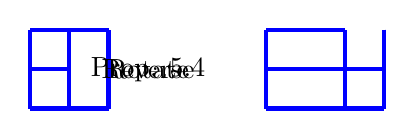
\begin{tikzpicture}
\tikzset{
    % Style for the dots
    dot/.style={
        circle,
        inner sep=1pt,
        fill=black,
        node contents={}
    },
    % Style for the lines
    myline/.style={
        draw=blue,
        ultra thick
    }
}
\begin{scope}[local bounding box=left]
	\draw[myline] (0,0)--(0,.5);
	\draw[myline] (.5,0)--(1,0);
	\draw[myline] (1,0)--(1,1);
	\draw[myline] (1,1)--(0,1);
	\draw[myline] (0,1)--(0,.5);
	\draw[myline] (.5,.5)--(0,.5);
	\draw[myline] (0,0)--(.5,0);
	\draw[myline] (.5,1)--(.5,.5);
	\draw[myline] (.5,0)--(.5,.5);
	\draw[myline] (.5,1)--(.5,.5);
	\node at (1.5,.5){Prop. 5.4};
	\draw[myline] (3,0)--(3,.5);
	\draw[myline] (3.5,0)--(4,0);
	\draw[myline] (4,0)--(4,1);
	\draw[myline] (4,1)--(3,1);
	\draw[myline] (3,1)--(3,.5);
	\draw[myline] (4.5,.5)--(3,.5);
	\draw[myline] (3,0)--(4.5,0);
	\draw[myline] (4.5,1)--(4.5,.5);
	\draw[myline] (4.5,0)--(4.5,.5);
	\draw[myline] (4.5,1)--(4.5,.5);
\end{scope}

\begin{scope}[local bounding box=middle]
	\draw[myline] (0,0)--(0,.5);
	\draw[myline] (.5,0)--(1,0);
	\draw[myline] (1,0)--(1,1);
	\draw[myline] (1,1)--(0,1);
	\draw[myline] (0,1)--(0,.5);
	\draw[myline] (.5,.5)--(0,.5);
	\draw[myline] (0,0)--(.5,0);
	\draw[myline] (.5,1)--(.5,.5);
	\draw[myline] (.5,0)--(.5,.5);
	\draw[myline] (.5,1)--(.5,.5);
	\node at (1.5,.5){Rotate};
	\draw[myline] (3,0)--(3,.5);
	\draw[myline] (3.5,0)--(4,0);
	\draw[myline] (4,0)--(4,1);
	\draw[myline] (4,1)--(3,1);
	\draw[myline] (3,1)--(3,.5);
	\draw[myline] (4.5,.5)--(3,.5);
	\draw[myline] (3,0)--(4.5,0);
	\draw[myline] (4.5,1)--(4.5,.5);
	\draw[myline] (4.5,0)--(4.5,.5);
	\draw[myline] (4.5,1)--(4.5,.5);
\end{scope}

\begin{scope}[local bounding box=right]
	\draw[myline] (0,0)--(0,.5);
	\draw[myline] (.5,0)--(1,0);
	\draw[myline] (1,0)--(1,1);
	\draw[myline] (1,1)--(0,1);
	\draw[myline] (0,1)--(0,.5);
	\draw[myline] (.5,.5)--(0,.5);
	\draw[myline] (0,0)--(.5,0);
	\draw[myline] (.5,1)--(.5,.5);
	\draw[myline] (.5,0)--(.5,.5);
	\draw[myline] (.5,1)--(.5,.5);
	\node at (1.5,.5){Reverse};
	\draw[myline] (3,0)--(3,.5);
	\draw[myline] (3.5,0)--(4,0);
	\draw[myline] (4,0)--(4,1);
	\draw[myline] (4,1)--(3,1);
	\draw[myline] (3,1)--(3,.5);
	\draw[myline] (4.5,.5)--(3,.5);
	\draw[myline] (3,0)--(4.5,0);
	\draw[myline] (4.5,1)--(4.5,.5);
	\draw[myline] (4.5,0)--(4.5,.5);
	\draw[myline] (4.5,1)--(4.5,.5);
\end{scope}

\end{tikzpicture}